\documentclass[aspectratio=169,10pt]{beamer}
\usepackage{amsmath,amssymb,booktabs,array,graphicx,tikz}
\usetikzlibrary{arrows.meta,positioning,shapes.geometric}

\definecolor{DeepNavy}{HTML}{17324D}
\definecolor{WarmCoral}{HTML}{E76F51}
\definecolor{SeaTeal}{HTML}{2A9D8F}
\definecolor{SoftGold}{HTML}{E9C46A}
\definecolor{WarmCream}{HTML}{F8F5EF}
\definecolor{Slate}{HTML}{5D6D7E}
\definecolor{PaleBlue}{HTML}{E8F0F4}

\usetheme{default}
\setbeamertemplate{navigation symbols}{}
\setbeamertemplate{headline}{}
\setbeamercolor{background canvas}{bg=WarmCream}
\setbeamercolor{normal text}{fg=DeepNavy,bg=WarmCream}
\setbeamercolor{structure}{fg=SeaTeal}
\setbeamercolor{frametitle}{fg=DeepNavy,bg=WarmCream}
\setbeamercolor{block title}{fg=white,bg=DeepNavy}
\setbeamercolor{block body}{fg=DeepNavy,bg=PaleBlue}
\setbeamerfont{frametitle}{size=\Large,series=\bfseries}
\setbeamerfont{title}{series=\bfseries}
\setbeamersize{text margin left=8mm,text margin right=8mm}
\setbeamertemplate{itemize item}{\color{WarmCoral}\scriptsize$\blacktriangleright$}
\setbeamertemplate{itemize subitem}{\color{SeaTeal}\tiny$\blacktriangleright$}
\setbeamertemplate{frametitle}{%
  \vspace{3mm}\insertframetitle\par\vspace{1mm}%
  {\color{SoftGold}\rule{\textwidth}{0.8pt}}\vspace{-1mm}}
\setbeamertemplate{footline}{%
  \leavevmode%
  \hbox{%
  \begin{beamercolorbox}[wd=.78\paperwidth,ht=3ex,dp=1.2ex,leftskip=8mm]{author in head/foot}%
    \color{Slate}\scriptsize Cooperative UAV-UGV Mission Planning
  \end{beamercolorbox}%
  \begin{beamercolorbox}[wd=.22\paperwidth,ht=3ex,dp=1.2ex,rightskip=6mm plus1fil]{date in head/foot}%
    \color{DeepNavy}\scriptsize\hfill\insertframenumber\,/\,\inserttotalframenumber
  \end{beamercolorbox}}}

\newcommand{\resultbox}[2]{%
\begin{beamercolorbox}[rounded=true,sep=1.5mm,wd=\linewidth]{block body}%
{\color{WarmCoral}\bfseries #1}\par{\small #2}
\end{beamercolorbox}}
\newcommand{\plainnote}[1]{%
\begin{beamercolorbox}[rounded=true,sep=1.5mm,wd=\linewidth]{block body}%
\small #1
\end{beamercolorbox}}

\title{Learning Virtual-Slot Rendezvous Scheduling for Cooperative UAV-UGV Missions}
\author{Aditya Pachauri \and Jalendu Pandey \and Kostubh Birla}
\institute{Department of Information Technology\\Indian Institute of Information Technology, Allahabad}
\date{}

\begin{document}

{
\setbeamercolor{background canvas}{bg=DeepNavy}
\begin{frame}[plain]
\begin{columns}[c,onlytextwidth]
\column{.72\textwidth}
{\color{SoftGold}\rule{26mm}{2pt}}\par\vspace{5mm}
{\color{white}\fontsize{24}{29}\selectfont\bfseries
Learning Virtual-Slot Rendezvous Scheduling for Cooperative UAV-UGV Missions\par}
\vspace{5mm}
{\color{WarmCream}\large Research Methodology Project Review\par}
\vspace{9mm}
{\color{white}Aditya Pachauri\quad Jalendu Pandey\quad Kostubh Birla\par}
\vspace{3mm}
{\color{PaleBlue}\small Department of Information Technology\par
Indian Institute of Information Technology, Allahabad\par}
\column{.23\textwidth}
\centering
\begin{beamercolorbox}[rounded=true,sep=3mm,wd=32mm]{block body}
\centering
\includegraphics[width=25mm]{assets/iiita_logo.png}
\end{beamercolorbox}
\end{columns}
\end{frame}
}

\begin{frame}{1. The Operational Bottleneck}
\begin{columns}[T,onlytextwidth]
\column{.53\textwidth}
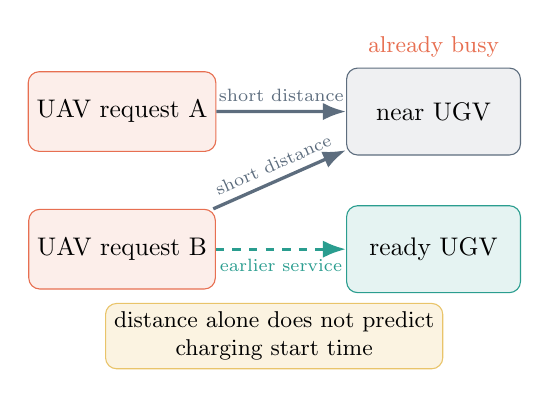
\begin{tikzpicture}[>=Latex,scale=.92,transform shape]
\node[draw=WarmCoral,fill=WarmCoral!12,rounded corners,minimum width=23mm,minimum height=11mm] (u1) at (0,2.3) {UAV request A};
\node[draw=WarmCoral,fill=WarmCoral!12,rounded corners,minimum width=23mm,minimum height=11mm] (u2) at (0,.4) {UAV request B};
\node[draw=Slate,fill=Slate!10,rounded corners,minimum width=24mm,minimum height=12mm] (g1) at (4.3,2.3) {near UGV};
\node[draw=SeaTeal,fill=SeaTeal!12,rounded corners,minimum width=24mm,minimum height=12mm] (g2) at (4.3,.4) {ready UGV};
\draw[->,very thick,Slate] (u1) -- node[above,sloped,font=\scriptsize]{short distance} (g1);
\draw[->,very thick,Slate] (u2) -- node[above,sloped,font=\scriptsize]{short distance} (g1);
\draw[->,very thick,SeaTeal,dashed] (u2) -- node[below,sloped,font=\scriptsize]{earlier service} (g2);
\node[align=center,font=\small,text=WarmCoral] at (4.3,3.2) {already busy};
\node[draw=SoftGold,fill=SoftGold!20,rounded corners,align=center,font=\small] at (2.1,-.8) {distance alone does not predict\\charging start time};
\end{tikzpicture}
\column{.43\textwidth}
\textbf{Mission setting}
\begin{itemize}
\item UAVs visit spatial tasks with limited energy.
\item UGVs move on roads and provide mobile charging.
\item Each UGV serves one UAV at a time.
\end{itemize}
\medskip
\textbf{Base-style decision [1]}
\[
j_i=\arg\min_j\|p_i^{\mathrm{land}}-p_j^{\mathrm{UGV}}\|_2
\]
\plainnote{A nearby charger can be the slow choice when its queue is long.}
\end{columns}
\end{frame}

\begin{frame}{2. From Nearest Charger to Scheduled Rendezvous}
\begin{columns}[T,onlytextwidth]
\column{.46\textwidth}
\begin{block}{Reference policy}
\begin{itemize}
\item A Transformer builds energy-feasible routes.
\item Recharge requests use nearest physical UGV assignment.
\item Service order is learned, but availability is not explicit.
\end{itemize}
\end{block}
\column{.46\textwidth}
\begin{block}{Virtual-slot policy}
\begin{itemize}
\item The same mission state produces landing requests.
\item Requests are matched to ordered UGV service positions.
\item Ready time and predicted waiting change each score.
\end{itemize}
\end{block}
\end{columns}
\vspace{1mm}
\resultbox{Research question}{Does joint routing and learned virtual-slot scheduling reduce completion-aware mission cost compared with the local proximity policy?}
\vspace{1mm}
{\small The design connects cooperative routing [1,2], multi-robot allocation [3], and structured matching [4].}
\end{frame}

\begin{frame}{3. Mission Model and Generated Instances}
\begin{columns}[T,onlytextwidth]
\column{.57\textwidth}
\centering
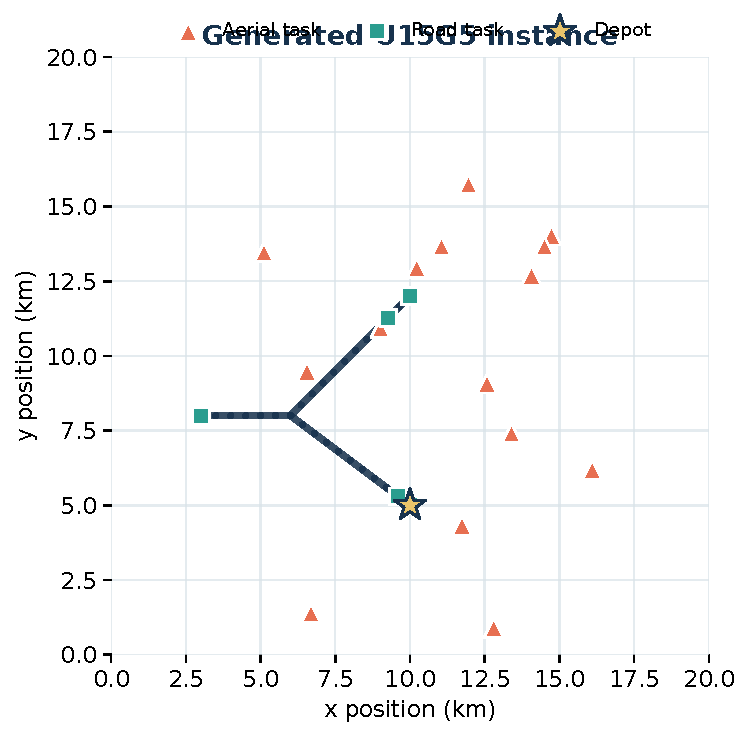
\includegraphics[width=\linewidth,height=55mm,keepaspectratio]{assets/scenario_v2.pdf}
\column{.39\textwidth}
\small
\begin{tabular}{@{}ll@{}}
\toprule
Workspace & $20\times20$ km\\
UAV speed & $10$ m/s\\
UGV speed & $4.5$ m/s\\
UAV capacity & $287.7$ kJ\\
Charging time & $15$ min\\
Sampling radius & $7$ km\\
\bottomrule
\end{tabular}
\medskip
\begin{itemize}
\item Seed changes task points and depot.
\item The three-branch road network stays fixed.
\item Baseline and proposed policies see the same test instance.
\item Flight, road travel, waiting, and serial charging are timed.
\end{itemize}
\end{columns}
\end{frame}

\begin{frame}{4. End-to-End Decision Pipeline}
\centering
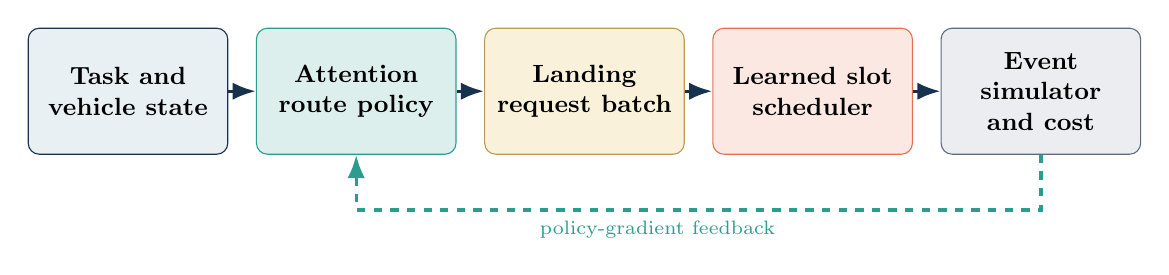
\begin{tikzpicture}[>=Latex,node distance=3.5mm,
stage/.style={draw,rounded corners,align=center,text width=23mm,minimum height=16mm,font=\small\bfseries}]
\node[stage,fill=PaleBlue,draw=DeepNavy] (state) {Task and vehicle state};
\node[stage,fill=SeaTeal!16,draw=SeaTeal,right=of state] (route) {Attention route policy};
\node[stage,fill=SoftGold!24,draw=SoftGold!80!black,right=of route] (requests) {Landing request batch};
\node[stage,fill=WarmCoral!16,draw=WarmCoral,right=of requests] (schedule) {Learned slot scheduler};
\node[stage,fill=Slate!12,draw=Slate,right=of schedule] (sim) {Event simulator and cost};
\draw[->,very thick,DeepNavy] (state)--(route);
\draw[->,very thick,DeepNavy] (route)--(requests);
\draw[->,very thick,DeepNavy] (requests)--(schedule);
\draw[->,very thick,DeepNavy] (schedule)--(sim);
\draw[->,very thick,SeaTeal,dashed] (sim.south) -- ++(0,-7mm)
  -| node[pos=.28,below,font=\scriptsize]{policy-gradient feedback} (route.south);
\end{tikzpicture}
\vspace{8mm}
\begin{columns}[T,onlytextwidth]
\column{.48\textwidth}
\textbf{Route stage}
\begin{itemize}
\item Three Transformer layers, width 128, eight heads [5].
\item Feasibility mask protects enough energy for rendezvous.
\item Output gives task choices and recharge requests.
\end{itemize}
\column{.48\textwidth}
\textbf{Scheduling stage}
\begin{itemize}
\item State MLPs create request and UGV embeddings.
\item Virtual slots represent future service order.
\item Hungarian matching gives a feasible test-time schedule [4].
\end{itemize}
\end{columns}
\end{frame}

\begin{frame}{5. Inside the Rendezvous Scheduler}
\begin{columns}[T,onlytextwidth]
\column{.54\textwidth}
\textbf{Virtual-slot compatibility}
\[
S_{i,(j,k)}=\frac{q_i^\top k_{j,k}}{\sqrt d}
-\gamma\frac{\widehat Q_{i,j,k}}{T_R}
\]
\[
\widehat Q_{i,j,k}=\max(0,r_j+t^{\mathrm{road}}_{ji}-t_i)+(k-1)T_R
\]
\begin{itemize}
\item $i$ identifies a UAV landing request.
\item $(j,k)$ is service position $k$ on physical UGV $j$.
\item The output selects a physical charger and an order.
\end{itemize}
\column{.42\textwidth}
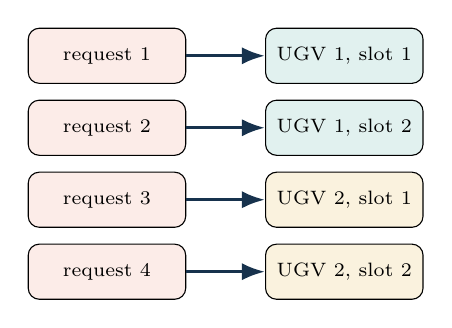
\begin{tikzpicture}[>=Latex,node distance=2mm,
cell/.style={draw,rounded corners,minimum width=20mm,minimum height=7mm,font=\scriptsize}]
\node[cell,fill=WarmCoral!13] (r1) {request 1};
\node[cell,fill=WarmCoral!13,below=of r1] (r2) {request 2};
\node[cell,fill=WarmCoral!13,below=of r2] (r3) {request 3};
\node[cell,fill=WarmCoral!13,below=of r3] (r4) {request 4};
\node[cell,fill=SeaTeal!14,right=10mm of r1] (s1) {UGV 1, slot 1};
\node[cell,fill=SeaTeal!14,below=of s1] (s2) {UGV 1, slot 2};
\node[cell,fill=SoftGold!22,below=of s2] (s3) {UGV 2, slot 1};
\node[cell,fill=SoftGold!22,below=of s3] (s4) {UGV 2, slot 2};
\draw[->,very thick,DeepNavy] (r1)--(s1);
\draw[->,very thick,DeepNavy] (r2)--(s2);
\draw[->,very thick,DeepNavy] (r3)--(s3);
\draw[->,very thick,DeepNavy] (r4)--(s4);
\end{tikzpicture}
\vspace{2mm}
\plainnote{Slots are queue positions. They do not create extra UGVs or extra chargers.}
\end{columns}
\end{frame}

\begin{frame}{6. How the Comparison Was Run}
\begin{columns}[T,onlytextwidth]
\column{.45\textwidth}
\textbf{Nine separately selected policy pairs}
\medskip
\begin{tabular}{lccc}
\toprule
 & 2U1G & 2U2G & 4U2G\\
\midrule
U15G5 & $\checkmark$ & $\checkmark$ & $\checkmark$\\
U45G15 & $\checkmark$ & $\checkmark$ & $\checkmark$\\
U75G25 & $\checkmark$ & $\checkmark$ & $\checkmark$\\
\bottomrule
\end{tabular}
\vspace{5mm}
\plainnote{Each pair uses 256 shared test scenarios. Task points differ across scenarios.}
\column{.51\textwidth}
\textbf{Recorded training schedule}
\begin{itemize}
\item Baseline uses 500 teacher updates and 300 policy-gradient updates.
\item Proposed policy starts from the baseline and receives 1,000 joint updates.
\item Four generated missions form one update.
\item Validation uses 256 scenarios per cell.
\item One main training seed is available per cell.
\end{itemize}
\medskip
{\color{WarmCoral}\bfseries Interpretation boundary}\par
\small This is a complete-policy comparison. Extra proposed training means the head-only causal effect is not isolated.
\end{columns}
\end{frame}

\begin{frame}{7. Primary Evidence as Paired Mission Costs}
\centering
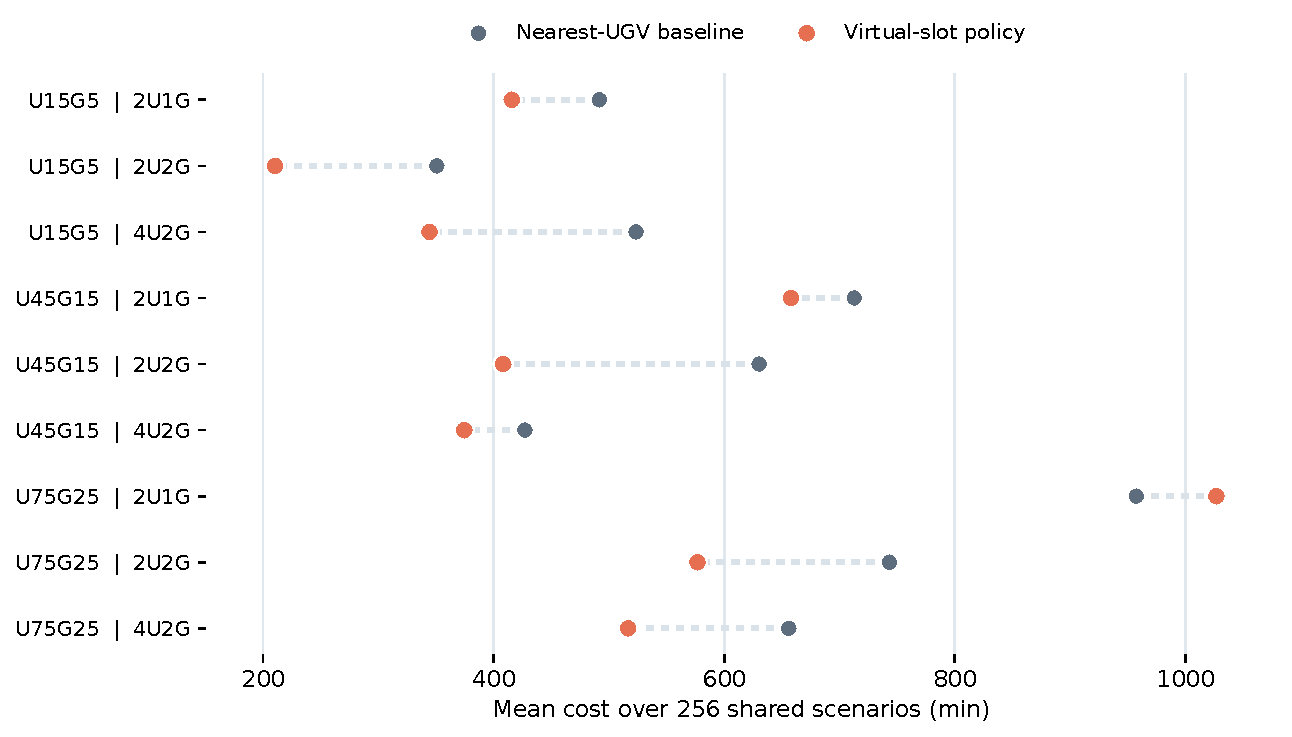
\includegraphics[width=.91\textwidth,height=59mm,keepaspectratio]{assets/cost_pairs.pdf}
\vspace{-1mm}
\plainnote{Cost equals mission makespan plus an 800-minute failure penalty. Lower values are better.}
\end{frame}

\begin{frame}{8. The Same Evidence Ranked by Relative Change}
\centering
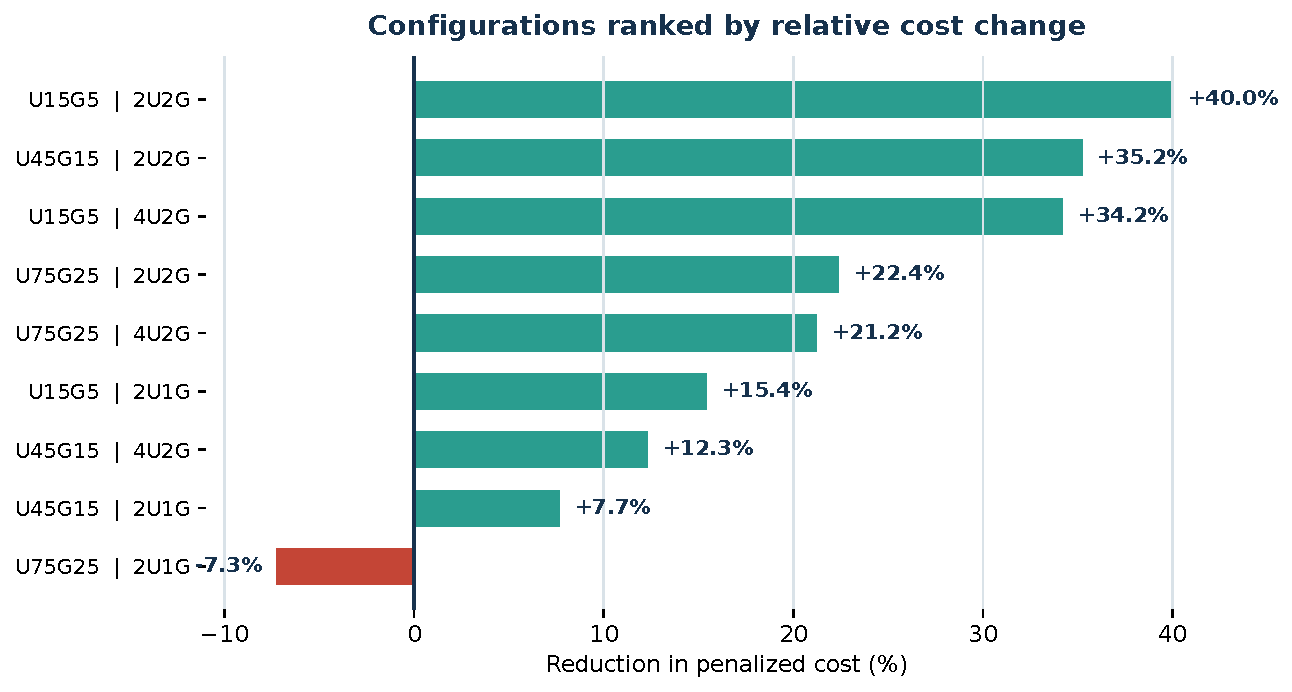
\includegraphics[width=.90\textwidth,height=53mm,keepaspectratio]{assets/gain_ranked.pdf}
\vspace{-1mm}
\resultbox{Observed outcome}{Eight of nine configurations have lower penalized cost. The largest reduction is 40.0 percent. U75G25 with 2U1G is the adverse case.}
\end{frame}

\begin{frame}{9. Where Landing Wait Changes}
\centering
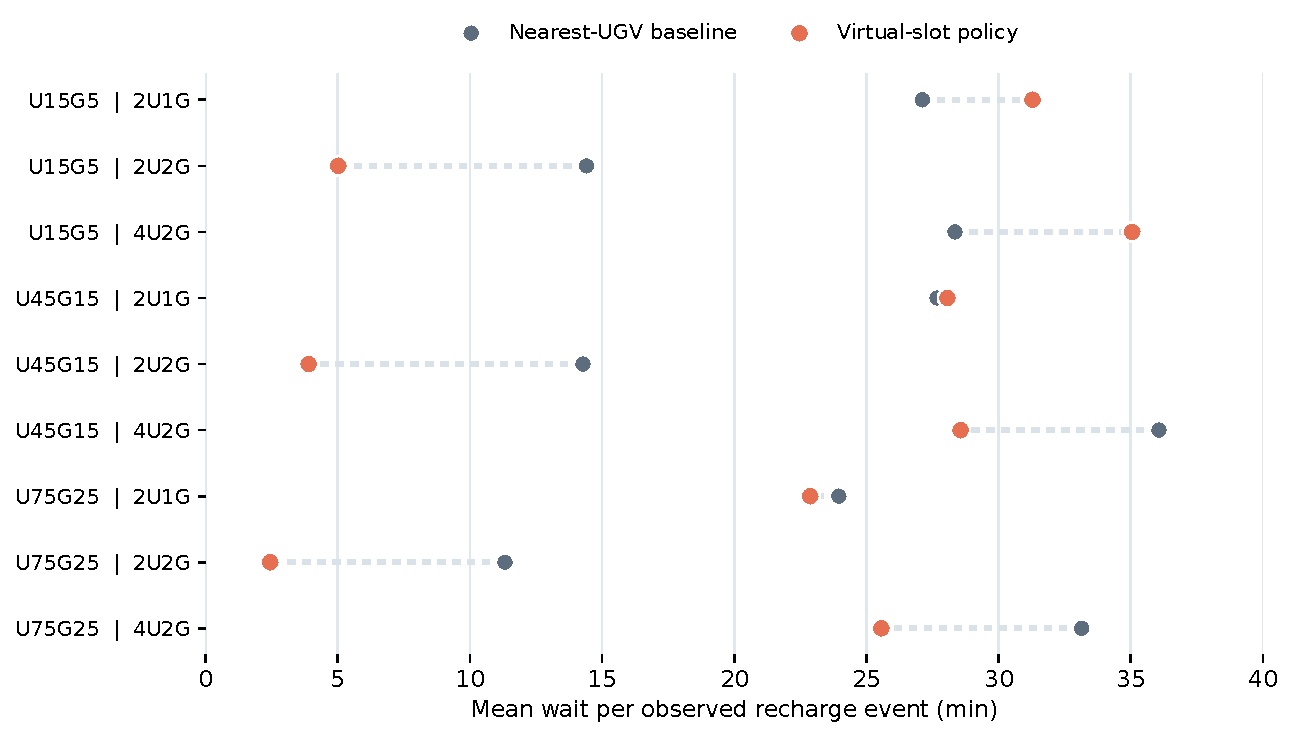
\includegraphics[width=.91\textwidth,height=57mm,keepaspectratio]{assets/wait_pairs.pdf}
\vspace{-1mm}
\plainnote{Wait per event falls in six cells. U15G5 with 4U2G has higher event wait but far fewer recharge events, so total wait per UAV and mission cost still fall.}
\end{frame}

\begin{frame}{10. Two Chargers Share Work More Evenly}
\centering
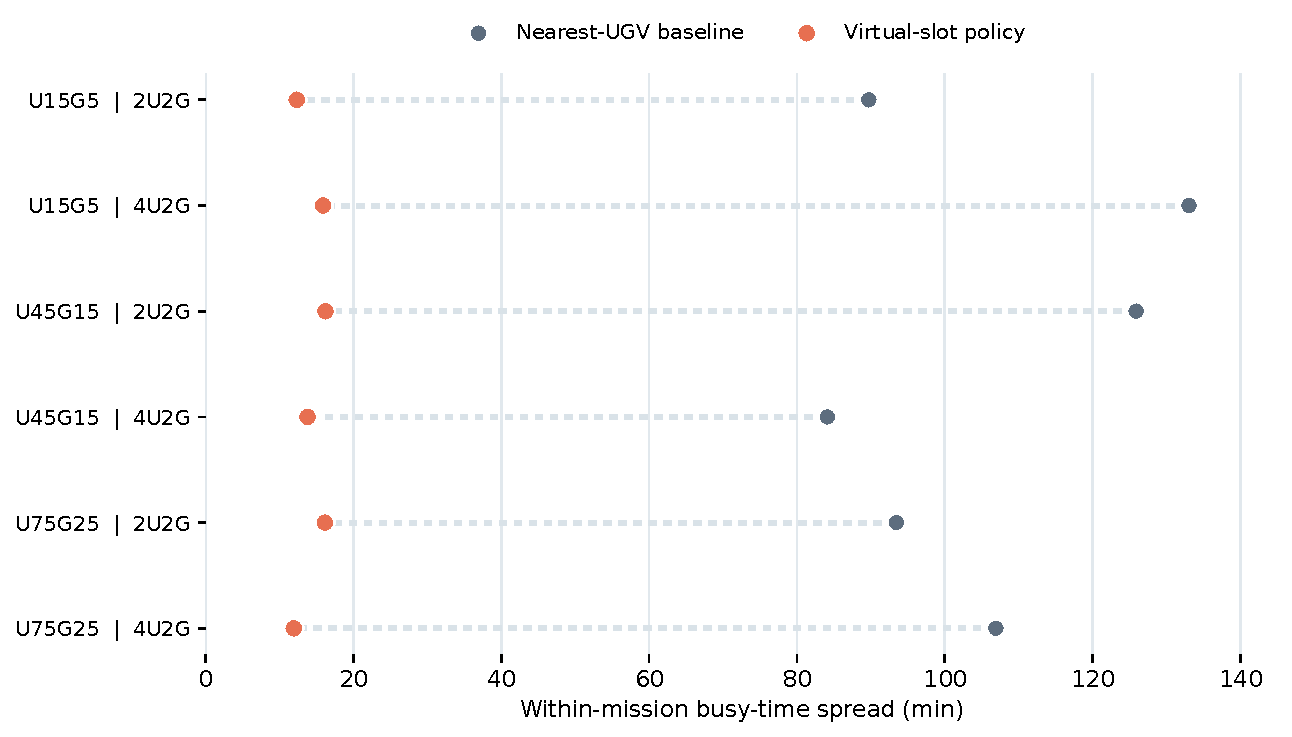
\includegraphics[width=.91\textwidth,height=52mm,keepaspectratio]{assets/load_pairs.pdf}
\vspace{-1mm}
\resultbox{Consistent operational effect}{Busy-time spread falls in all six two-UGV configurations. Lower spread means road travel and charging work are distributed more evenly.}
\end{frame}

\begin{frame}{11. Reliability and Computation}
\begin{columns}[T,onlytextwidth]
\column{.68\textwidth}
\centering
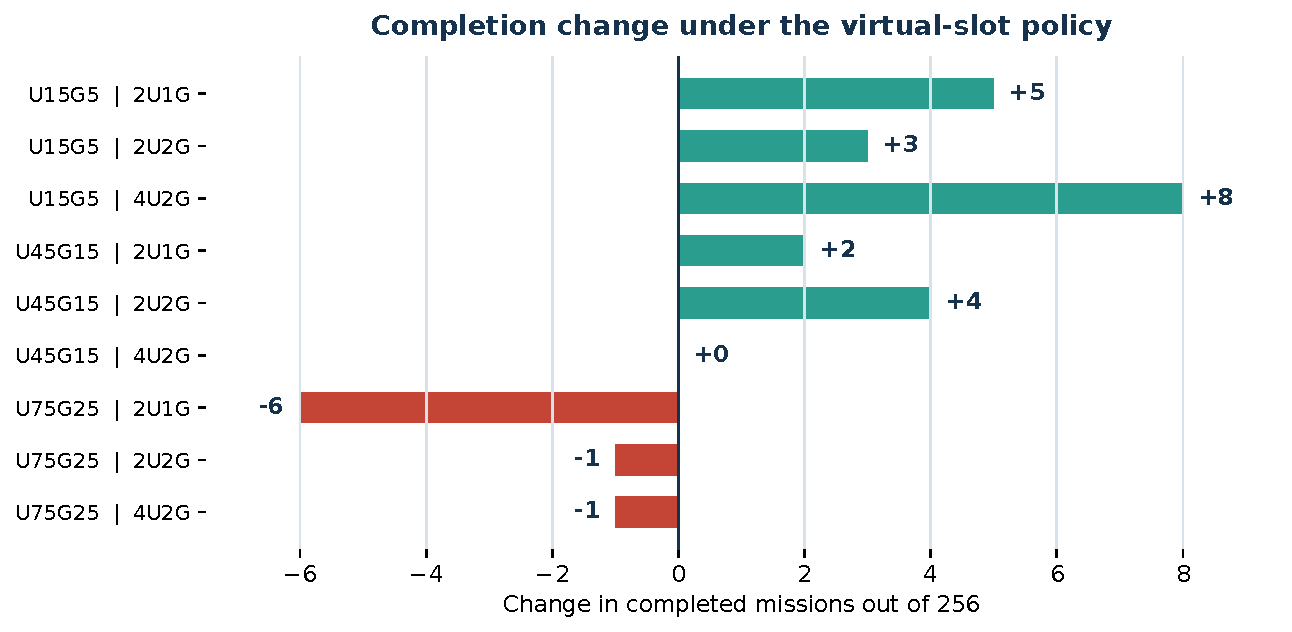
\includegraphics[width=\linewidth,height=56mm,keepaspectratio]{assets/completion_delta.pdf}
\column{.28\textwidth}
\resultbox{38 to 24}{Total failures decrease across the full matrix.}
\vspace{3mm}
\resultbox{5.46 to 15.16 ms}{Mean proposed CPU planning time per recharge round.}
\vspace{3mm}
\plainnote{U75G25 with 2U1G loses six completions and remains the main failure case.}
\end{columns}
\end{frame}

\begin{frame}{12. What the Ablations Tell Us}
\begin{columns}[T,onlytextwidth]
\column{.58\textwidth}
\centering
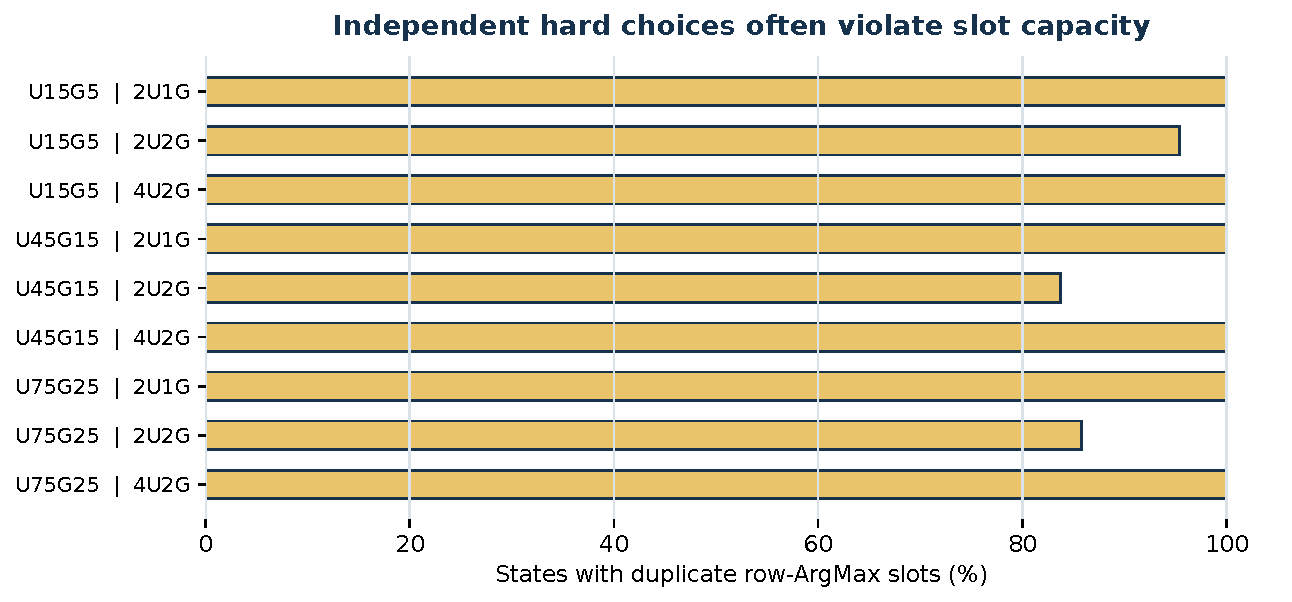
\includegraphics[width=\linewidth,height=55mm,keepaspectratio]{assets/collision_rates.pdf}
\column{.38\textwidth}
\textbf{Three separate checks}
\begin{itemize}
\item Learned $\gamma$ beats retrained $\gamma=0$ in mean cost for eight cells, but routes also change.
\item A frozen queue toggle has no effect with one UGV, as expected from slot symmetry.
\item Hard row ArgMax frequently gives duplicate slots.
\end{itemize}
\plainnote{The ablations support capacity-aware decoding. They do not prove that soft training always gives lower validation cost.}
\end{columns}
\end{frame}

\begin{frame}{13. Answer to the Research Question}
\begin{columns}[T,onlytextwidth]
\column{.48\textwidth}
\begin{block}{What was achieved}
\begin{itemize}
\item A working 2D cooperative mission simulator.
\item Learned routing with feasible virtual-slot matching.
\item Nine paired policy comparisons and targeted ablations.
\item Lower cost in 8 of 9 tested configurations.
\end{itemize}
\end{block}
\column{.48\textwidth}
\begin{block}{What remains}
\begin{itemize}
\item Equal training budgets and repeated full-policy seeds.
\item Strong availability-based scheduling baselines.
\item New road networks and larger fleets.
\item Higher-fidelity docking and motion tests.
\end{itemize}
\end{block}
\end{columns}
\vspace{4mm}
\resultbox{Conclusion}{Within the evaluated simulator and training setup, learned joint routing and virtual-slot scheduling improves mission efficiency and balances two-UGV charging work better than the local proximity policy.}
\end{frame}

\begin{frame}{References}
\small
\begin{enumerate}
\item M. S. Mondal, S. Ramasamy, and P. Bhounsule. ``How to Coordinate UAVs and UGVs for Efficient Mission Planning?'' Robotics, Science and Systems, 2025.
\item P. Maini, K. Sundar, M. Singh, S. Rathinam, and P. B. Sujit. ``Cooperative Aerial-Ground Vehicle Route Planning With Fuel Constraints for Coverage Applications.'' IEEE Transactions on Aerospace and Electronic Systems, 2019.
\item B. P. Gerkey and M. J. Matari\'c. ``A Formal Analysis and Taxonomy of Task Allocation in Multi-Robot Systems.'' The International Journal of Robotics Research, 2004.
\item H. W. Kuhn. ``The Hungarian Method for the Assignment Problem.'' Naval Research Logistics Quarterly, 1955.
\item W. Kool, H. van Hoof, and M. Welling. ``Attention, Learn to Solve Routing Problems!'' ICLR, 2019.
\end{enumerate}
\vfill
{\color{Slate}\scriptsize Numerical results come from the preserved nine-cell aggregate evaluation. Both policies use the same 256 test scenarios inside each cell.}
\end{frame}

\end{document}
